% 20 Apr 2014 : GWA : 3 pages.

\section{Design}
\label{sec-design}

A PocketLocker personal storage cloud (PSC) consists of a set of
clients---including smartphones, tablets, laptops, desktops, and dedicated
storage appliances---and a cloud service called the \textit{orchestrator}.
Like most filesystems, PocketLocker uses a namespace to map paths to a set of
$n$ uniquely-identified \textit{chunks} containing file data. Because chunks
are the output of erasure coding, the number of distinct chunks required for
reconstruction $k$ is less than $n$, and $k$ is stored in the namespace for
each path.

The orchestrator maintains the authoritative namespace by using a
monotonically-increasing counter to version all namespace modifications,
including opens, renames, updates, and deletes. It also fixes the location of
certain chunks to meet backup requirements and coordinates transfers between
firewalled clients during open. While the orchestrator must track the
location of some chunks to meet backup requirements, it does not maintain the
location of all chunks. The orchestrator only requires a small amount of
storage to facilitate transfers between firewalled PSC clients.

Clients contribute storage to the PSC which PocketLocker divides into a
\textit{file cache}, used to store reconstructed files, and a \textit{chunk
store}, used to store chunks. By applying updates from the orchestrator
clients maintain a local cache of the namespace to efficiently perform path
lookups. Clients also track what chunks for each path they have in their local
chunk store. PocketLocker users configure several attributes when attaching
clients:

\begin{enumerate}
  
  \item \textbf{Capacity.} The storage a client contributes to the PSC
   
  \item \textbf{Backup.} Whether the client should be used to meet PSC backup
    requirements. If so, it's failure may lead to data loss. PocketLocker
    uses this attribute when determining where to backup chunks.

  \item \textbf{Availability.} Whether files stored on the PSC can be
    unavailable when the client is unreachable. PocketLocker uses this
    attribute when determining where to store chunks so that files remain
    available.

  \item \textbf{Interactivity.} Whether files are created or accessed on this
    client. PocketLocker uses this attribute when reclaiming storage.

  \item \textbf{Power.} Whether the client is battery- or wall-powered.
    PocketLocker uses this attribute when acquiring chunks during open.

\end{enumerate}

PocketLocker provides example sets of configuration options for common types
of devices. A NAS appliance would be used for backup and availability,
non-interactive and wall-powered. A laptop would be used for backup but not
for availability, interactive and battery-powered. A smartphone would not be
used for backup or availability, interactive and battery-powered. A desktop
would be used for backup, interactive and wall-powered, and could or could
not be used for availability depending on whether it was regularly shut off
and whether the user cared if they were able to access their PSC when it was.

\subsection{Creating, Modifying, and Deleting Files}

\begin{figure}[t]

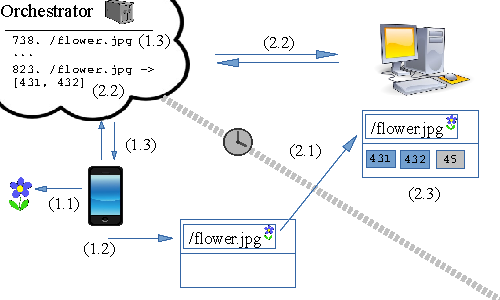
\includegraphics[width=\columnwidth]{./figures/create.pdf}

\caption{\small \textbf{Creation.} This illustrates (1) path registration,
performed immediately by a battery-powered client; and (2) erasure coding
and chunk registration, performed later by a wall-powered client.}

\label{fig-design-creation}

\end{figure}

To reduce energy usage on battery-powered clients, PocketLocker separates
creation into two steps which can be performed on different clients: (1) path
registration, a lightweight operation; and (2) erasure coding and chunk
registration, a heavyweight operation. Figure~\ref{fig-design-creation}
illustrates the process. When a file is created the creator moves the file
into its file cache (1.1) and immediately registers the path with the
orchestrator (1.2), which immediately publishes it to other clients to avoid
path collisions (1.3). During the second part of creation, once the file is
erasure coded (2.1) $n$ new chunks will be created and registered with the
in setting up our experiments and providing information about the testbed.
orchestrator, which assign them unique IDs and associates the set of IDs with
the path (2.2). The client then moves the chunks into its chunk store (2.3).
Battery-power clients will wait to transfer the file for a period of time
configured as part of the backup process, described later in
Section~\ref{subsec-backup}.

Modifications to existing PocketLocker files create a new version of a file.
They require an additional round of erasure coding and distribution of new chunks.
Because updating files is a heavyweight operation,
PocketLocker is designed for files that are rarely or never changed, such as
the media files in our traces of which were almost never altered. Renames
simply alter the path associated with existing chunks, and deletes removes
the path from the namespace.

Both updates and deletions invalidate chunks which clients add to a
reclamation list, but chunks are not removed until storage is needed. Because
clients do not coordinate chunk removal with the orchestrator, PocketLocker
provides no guarantees about the existence of old version or deleted files.
However, because the reclamation list is processed in FIFO order,
modifications are generally removed first. Providing stronger semantics would
require more coordination between clients and the orchestrator which we have
chosen to avoid.

\subsection{Opening Files}

\begin{figure}[t]

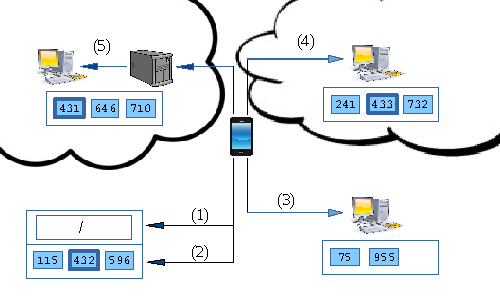
\includegraphics[width=\columnwidth]{./figures/open.pdf}

\caption{\small \textbf{Open.} The figure illustrates a case where the
request is satisfied by locating k=3 chunks:  one in the client's local
chunk store, and two on PSC devices in the WAN.}

\label{fig-design-open}

\end{figure}

To open a file, the opener first verifies that the path is valid. If the file
is already in the file cache, the open completes immediately. Otherwise, the
client maps the path to the $n$ chunk IDs and locates $k$ as follows:

\begin{enumerate}

\item \textbf{Local chunk store.} If the opener has $k$ chunks of the file in
its chunk store it reconstructs the file and adds it to its file cache.
%
\label{itemize-local}

\item \textbf{LAN transfer.} If the opener is on a LAN with other PSC clients
it will broadcast a \textit{chunk request} identifying the path and chunks it
needs to its LAN PSC neighbors which will each report which requested chunks
they store. PocketLocker clients discover neighbors using a simple UDP
broadcast. Based on the replies the opener will acquire any needed chunks and
add them to its chunk store. If it has $k$ chunks, then the open continues as
in Step~\ref{itemize-local}.

As an optimization, if an opener requests $k$ chunks for a path and a PSC
neighbor has the reconstructed file in its file cache, it will offer to
transfer the file instead of chunks. This optimization is also applied in
Steps~\ref{itemize-wan}~and~\ref{itemize-orchestrator}.
%
\label{itemize-lan}

\item \textbf{WAN transfer.} If the opener has not acquired $k$ chunks after
Step~\ref{itemize-lan}, it forwards the remaining request to other reachable
PSC clients and processes replies as in Step~\ref{itemize-lan}.
%
\label{itemize-wan}

\item \textbf{Orchestrated transfer.} If at the end of Step~\ref{itemize-wan}
the opener still does not have $k$ chunks, it forwards the remaining request
to the orchestrator. At this point the orchestrator may be able to facilitate
transfers with clients not publicly reachable in Step~\ref{itemize-wan}, or
the open may fail.
%
\label{itemize-orchestrator}

\end{enumerate}

Figure~\ref{fig-design-open} highlights the above process.  The client needs
chunks 431-433 to reconstruct a file.  The client first checks its local
cache (1) and is unable to locate the file.  It is, however, able to locate
chunk 432 in its own chunk store (2).  A search of LAN devices does not turn
up any of the desired chunks (3), but the client finds chunk 433 on a WAN
device (4).  Finally, the Orchestrator is able to locate the last chunk, 431,
on another WAN device (5).

PocketLocker reduces energy consumption at battery-powered clients in two
ways. First, it allows them to delegate opens to a wall-powered client which
receives a delegated chunk request and then proceeds as in
Step~\ref{itemize-lan}: issuing any additional chunk requests on the
battery-powered client's behalf and transferring all chunks to the opener when
the open completes. Second, all clients will prefer to transfer chunks from
wall-powered clients in Steps~\ref{itemize-lan}~and~\ref{itemize-wan}.

Depending on where required chunks are located, opening a file
can take a variable amount of time.  We allow apps
to request a notification if an open may require more than a configurable
amount of time, allowing them to notify the user or move themselves
temporarily into the background until the required transfers complete.

Finally, PSC clients can request files as soon as they receive the path
creation notification, meaning that this can occur before the file has been
erasure coded and the chunks registered. In this case the open request only
specifies the path, and clients reply if they have the file in their file
cache. Normally the file creator will be the only PSC client with the file
and required to transfer it to the opener. If the opener is wall-powered, it
then performs the erasure coding and creation continues as described
previously. We expect that in most cases when files are requested before they
have been erasure coded, the user has moved the creator onto the same LAN
with the opener---such as when a user tries to open a photo taken on their
smartphone on their laptop. If so, the time and energy required to transfer
the file to the opener should be minimal.

\subsection{Performance}

PocketLocker attempts to use all available client storage to enable
reliability, availability, and performance by intelligently locating chunks
within the PSC. PocketLocker reduces the latency of file accesses in two
ways. First, because many file accesses occur soon after the file is created,
PSC clients opportunistically acquire $k$ chunks of newly created files after
receiving creation notifications from the orchestrator. On wall-powered
clients this is done immediately; battery-powered clients wait until their
next charging session. To evenly distribute chunks between clients to help
meet later backup requirements, these chunk requests identify the path but
not the chunk IDs, allowing the client receiving the request to provide
distinct subsets of $k$ chunks of the $n$ available to different clients.
Initial chunk requests also disable the optimization described previously to
prevent the creator from transferring the reconstructed file rather than file
chunks.

Second, PSC clients track local file access patterns to intelligently manage
their local chunk store when reclaiming space. When under storage pressure,
after emptying their reclamation list, clients can either (1) remove
reconstructed files from their file cache or (2) remove chunks from their
chunk store. Because erasure decoding is more efficient than erasure
encoding, clients first remove files in their file cache such that they have
enough chunks in their chunk store to reconstruct.

At this point removing either files or chunks allows the client to make
latency tradeoffs between different files. For example, keeping one chunk of
many files reduces the access latency of all but provides low-latency access
to none\footnote{Note that wall-powered PocketLocker clients can also repeat
the erasure coding process to reconstruct missing chunks for files in their
file store, but do to the overhead of erasure coding battery-powered clients
will not.}; at the other extreme, keeping complete files---either in the file
store or as $k$ chunks---provides low-latency access to a smaller set of
files but higher latency for the rest. Because file chunk size varies,
removing one chunk of a large file can create more space than several chunks
of smaller files, but removing chunks of more files increases the probability
that a chunk will be required during open. We compare several algorithms for
reclaiming storage in Section~\ref{subsec-evaluation-traces} evaluating their
performance on our \PhoneLab{} file access traces.

Interactive and non-interactive clients reclaim storage differently.
Interactive clients keep statistics on their own chunk access patterns and
utilize them during reclamation, but do not track chunks transferred to other
devices in response to chunk requests. Because non-interactive clients do not
access files locally, they only keep statistics on chunks accessed to respond
to chunk requests. As a result, interactive clients optimize for their own
behavior, while non-interactive clients optimize for the clients they
interact with.

\subsection{Backup and Availability}
\label{subsec-backup}

\begin{figure}[t]

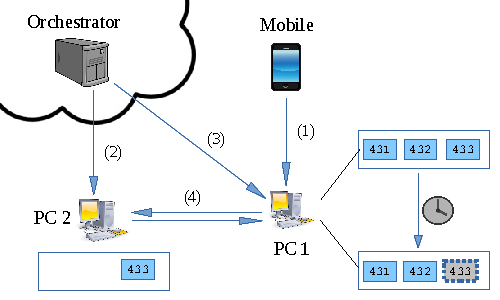
\includegraphics[width=\columnwidth]{./figures/backup.pdf}

\caption{\small \textbf{Backup.} A file is received and chunked by a powered
device.  Under the direction of the Orchestrator, pinned chunks are
distributed among different devices.}

\label{fig-design-backup}

\end{figure}

The orchestrator both meets backup requirements and ensures availability by
\textit{pinning} chunks at clients to ensure that $k$ chunks will always be
available---as long as the client configured as available are reachable---and
survive client failures. Pinning prevents clients from removing chunks during
reclamation. PocketLocker allows users to configure their PSC to not lose any
files older than a certain time interval (the backup window) if up to a
certain number of clients fail (the backup threshold).

Figure~\ref{fig-design-backup} shows the most common steps in the backup
process.  A powered device receives and chunks a file originally created by
a mobile device (3.1).  All chunks are initially pinned by default.  Next,
the Orchestrator orders PC 2 to request chunk 433 from PC 1 (3.2), and PC 1
to unpin chunk 433 after the chunk has been copied to PC 2 (3.3).  The clients
then carry out these instructions:  PC 1 fetches and pins chunk 433 from PC 2,
and PC 1 unpins chunk 433 (3.4). 

Backup and availability requirements can reduce the usable size of the PSC
depending on the distribution of storage contributed by clients and how they
are configured. For example, a single small client can limit the size of the
entire PSC if its storage must be used for backup. Or, a single large client
may find its storage underutilized if it is not marked as available.
PocketLocker estimates the capacity of the PSC at configuration time as the
lesser of (1) the sum of all the capacity contributed by clients marked as
available and (2) the sum of the storage contributed by the smallest backup
clients required to meet the backup threshold. The tradeoff between client
attributes and the PSC capacity is presented to the users when they configure
clients and choose their backup threshold. Remaining PSC space is not unused:
PocketLocker uses it to improve performance by caching chunks and
reconstructed files, and to allow users to recover deleted files and old file
versions.

When the orchestrator is unable to meet the backup or availability
requirements the PSC is full and new files cannot be created. The user is
warned when the PSC is nearing capacity and requested to add storage or
remove files. To allow file access, interactive clients reserve a portion of
their storage for the file cache; to allow chunk transfers, all clients
reserve a portion of their chunk store for unpinned chunks.

The backup window allows PocketLocker to reduce energy usage on
battery-powered clients by not forcing them to immediately transfer created
files to other PSC clients or receive pinned chunks required for backup. When
new files are created on battery-powered client, the client begins attempting
to offload the file to a wall-powered client, which will perform the second
part of the file creation process, including erasure coding and distributing
chunks to other clients. Our current algorithm waits a configurable portion
of the backup window for the device to be plugged in, and if that time window
expires it transfers the file as soon as it reaches an energy-efficient
network such as a wired or Wifi connection. When the backup window is about
to expire, any available connection---including mobile data networks---is used
as a last resort. Users are warned that short backup windows will produce
high energy consumption when configuring their backup window.

Users can report client failures to PocketLocker manually or configure
PocketLocker to consider a backup client as failed if the orchestrator cannot
reach it for a period of time. Once a new client has been attached to the PSC
after a failure, the orchestrator will immediately rerun the pinning
algorithm described in Section~\ref{sec-design-algorithm} which will cause
the new client to request chunks needed to meet the backup requirement. In
certain cases erasure coding may need to be repeated for some files to
recover the full set of $n$ chunks, but this can proceed using any $k$ chunks
that are available.

\subsection{Erasure Coding Parameters}

The erasure coding parameters affect the design of the PocketLocker PSC in
two ways. First, if $n$ is smaller than the number of backup clients then the
orchestrator may need to move a chunk from one client to another to rebalance
storage usage while meeting backup requirements. Since this is undesirable,
we choose $n$ to be equal to the number of devices initially configured for
backup.

Second, $k$ determines both the chunk size---which is equal to the file size
divided by $k$---and the overhead of erasure decoding, which increases with
$k$. Using larger values of $k$ and creating larger numbers of smaller chunks
allows more even storage distribution over clients, and allows clients to
make finer-granularity tradeoffs between storage and access latency by
caching between $1$ and $k$ chunks of the file in their chunk store. However,
due to PocketLocker's focus on supporting battery-powered clients, we set $k
= 2$ to minimize the energy overhead of erasure decoding.

\subsection{Chunk Pinning Algorithm}
\label{sec-design-algorithm}

Periodically the orchestrator collects a list of chunks they are storing from
all PSC clients and runs a \textit{chunk pinning algorithm} to determines
where to pin chunks to meet the user's backup and availability requirements.
Our current placement algorithm uses a greedy approach that meets the backup
requirements and availability requirements in separate passes. If the size of
the PSC is constrained by the backup requirement, the availability pass
proceeds first in order to avoid reducing capacity on clients needed for
backup. If the size of the PSC is constrained by the availability
requirement, the order of the two passes is reversed.

In each pass, for each file the orchestrator begins with the client with the
most capacity and begins pinning chunks until the requirement is met. The
backup pass stripes chunks across backup clients to meet the backup
requirement, while the availability pass stacks chunks onto available devices
to meet the availability requirement. The algorithm attempts to avoid chunk
transfers when possible by considering what chunks each client already has
pinned or available in their chunk store.

When clients receive a list of pinned chunks from the orchestrator, they
retrieve any chunks they are missing using the chunk request process
described previously. To ensure that chunks for newly-created files are not
evicted before they can be pinned by the orchestrator, chunks for new files
and file updates are initially pinned after creation at all clients. The next
time the backup algorithm runs, many of these chunks will be unpinned.

\subsection{Offline Operation}

PocketLocker assumes clients are connected most of the time, but can support
periods of disconnected operation. Disconnected clients can access any files
in their file store or that they can reconstruct using chunks in their local
chunk store. Any changes to the namespace, such as creations, are cached.
When the client reconnects, it downloads any namespace updates from the
orchestrator and identifies any conflicts which the user is required to
resolve locally. Because it is designed to store media files, PocketLocker
does not attempt to merge conflicting creations or modifications. Instead,
users are asked to choose between updates or rename the file.

\subsection{File Metadata}

Finally, to support media files that may require metadata for browsing, such
as photo thumbnails, PocketLocker allows metadata files up to a size limit to
be associated with files stored in the PSC. Metadata files are stored in a
separate part of each client's storage and retrieved during the initial chunk
requests that follow file creation. Unlike chunks, however, metadata files
are not reclaimed, since we assume that the overhead of storing them will be
limited.
